\chapter[Multi-Agent Reinforcement Learning]{Multi-Agent\\ Reinforcement Learning}
\label{chap: Multi-agent RL}
\vspace{1cm}

So far, we have only considered solving a single-pair shortest path problem using a single-agent reinforcement learning method. In this chapter, we discuss how to solve UMCFND problems using the reinforcement learning method while multiple agents acting in the same environment are allowed.

In section,

In section,

In section, 


\clearpage
\section{Cooperative Markov Game}
In UMCFND problems, each commodity $k \in \mathcal{K}$,  characterized by an origin node $O(k)$, destination node $D(k)$, and its quantity $d^k$, can be considered as an agent who makes its own path. Thus, UMCFND problems can be described as a Markov Game, which is a multi-agent extension of Markov decision processes (\citeauthor{littman1994markov} \cite{littman1994markov}).

Let $\mathcal{S}$ denote a finite set of global states $S_t$, shared by all agents. At each time step $t$, each agent, identified by $m \in \mathcal{M} = \{1, \dots, M\}$, simultaneously chooses an action $A_t^{(m)} \in \mathcal{A}^{(m)}(s) \subset \mathcal{A}^{(m)}$ available in state $S_t=s$. These actions $\{A_t^{(m)}\}_{m\in\mathcal{M}}$ form a joint action $Z_t$:
$$Z_t = (A_t^{(1)}, \dots, A_t^{(M)}) \in \mathcal{A}^{(1)}(s) \times \cdots \times \mathcal{A}^{(M)}(s) = \mathcal{Z}(s) \subset \mathcal{Z} =\mathcal{A}^{(1)}\times \cdots \times \mathcal{A}^{(M)}$$
Since the environment in UMCFND problems is deterministic as in the case of \hyperref[fig:toy graph]{Example 1}, we only consider a deterministic state-transition rule $\tau(s, z): \mathcal{S} \times \mathcal{Z} \rightarrow \mathcal{S}$. Furthermore, as the goal of UMCFND problems is to minimize the objective function \eqref{eq:obf}, a reward function $r(s,z): \mathcal{S} \times \mathcal{Z} \rightarrow \mathbb{R}$ is shared by all agents, implying that our Markov game is a \textit{cooperative} Markov Game.

Let $\Pi: \mathcal{S} \times \mathcal{Z} \rightarrow [0,1]$ denote a policy in the cooperative Markov Game:
\begin{align}
 \Pi(z|s):= \text{Pr}(Z_t = z \ | \ S_t = s), \quad \forall z \in \mathcal{Z}(s) \text{ for each } s\in \mathcal{S}
\end{align}
The objective of learning in the cooperative Markov game is to find an optimal policy $\Pi_\ast$, which is a policy that maximizes the discounted return $$\sum_{t=0}^\infty \gamma^t r(S_t,Z_t)$$

A single-agent reinforcement learning can be used to obtain such optimal policy by considering a whole team as a single agent. Q-learning for a cooperative Markov game, for instance, is described by the following update rule:
\begin{align}
    Q(S_t, Z_t) \leftarrow Q(S_t, Z_t) + \alpha\big[ r(S_t, Z_t) + \gamma \ \underset{z\in\mathcal{Z}(S_{t+1})}{\text{max }}Q(S_{t+1}, z) - Q(S_t, Z_t)\big],
\end{align}
As in \autoref{tab:Q(s,a)}, the action-value function estimate $Q(s,z)$ can be represented by a table of size $|\mathcal{S}| \times |\mathcal{Z}| = |\mathcal{S}| \times |\mathcal{A}^{(1)} \times \cdots \times \mathcal{A}^{(M)}|$. Thus, using Q-learning to solve a cooperative Markov game is vulnerable to scalability, since the size of table grows exponentially as the number of agent increases.

Moreover, as a single-agent reinforcement learning does not allow multiple agents, its learning procedure for an optimal policy in a  cooperative Markov game cannot be distributed among agents. In other words, a single-agent reinforcement learning method is restricted to a centralized-learning-centralized-execution which may be more inefficient than other learning structure, such as a centralized-learning-decentralized-execution. In the following sections, we discuss several methods using a centralized-learning-decentralized-execution structure, which is a current paradigm of multi-agent reinforcement learning(\citeauthor{zhang2019multi} \cite{zhang2019multi}).

\subsection{Example 2: UMCFND problem}
Throughout this chapter we consider an example of UMCFND problem where a directed graph $G = (V,E)$ is given as in \autoref{fig:Example2}, and $\mathcal{K} = \{1,2\}, \ O(1) = 6, \ O(2) = 7, \ D(1) = 9, \ D(2) = 10, \ d^1 = 10, \ d^2 = 15$.

\label{Example2}
\begin{figure}[hbt!]
    \centering
    \captionsetup{justification=centering}
    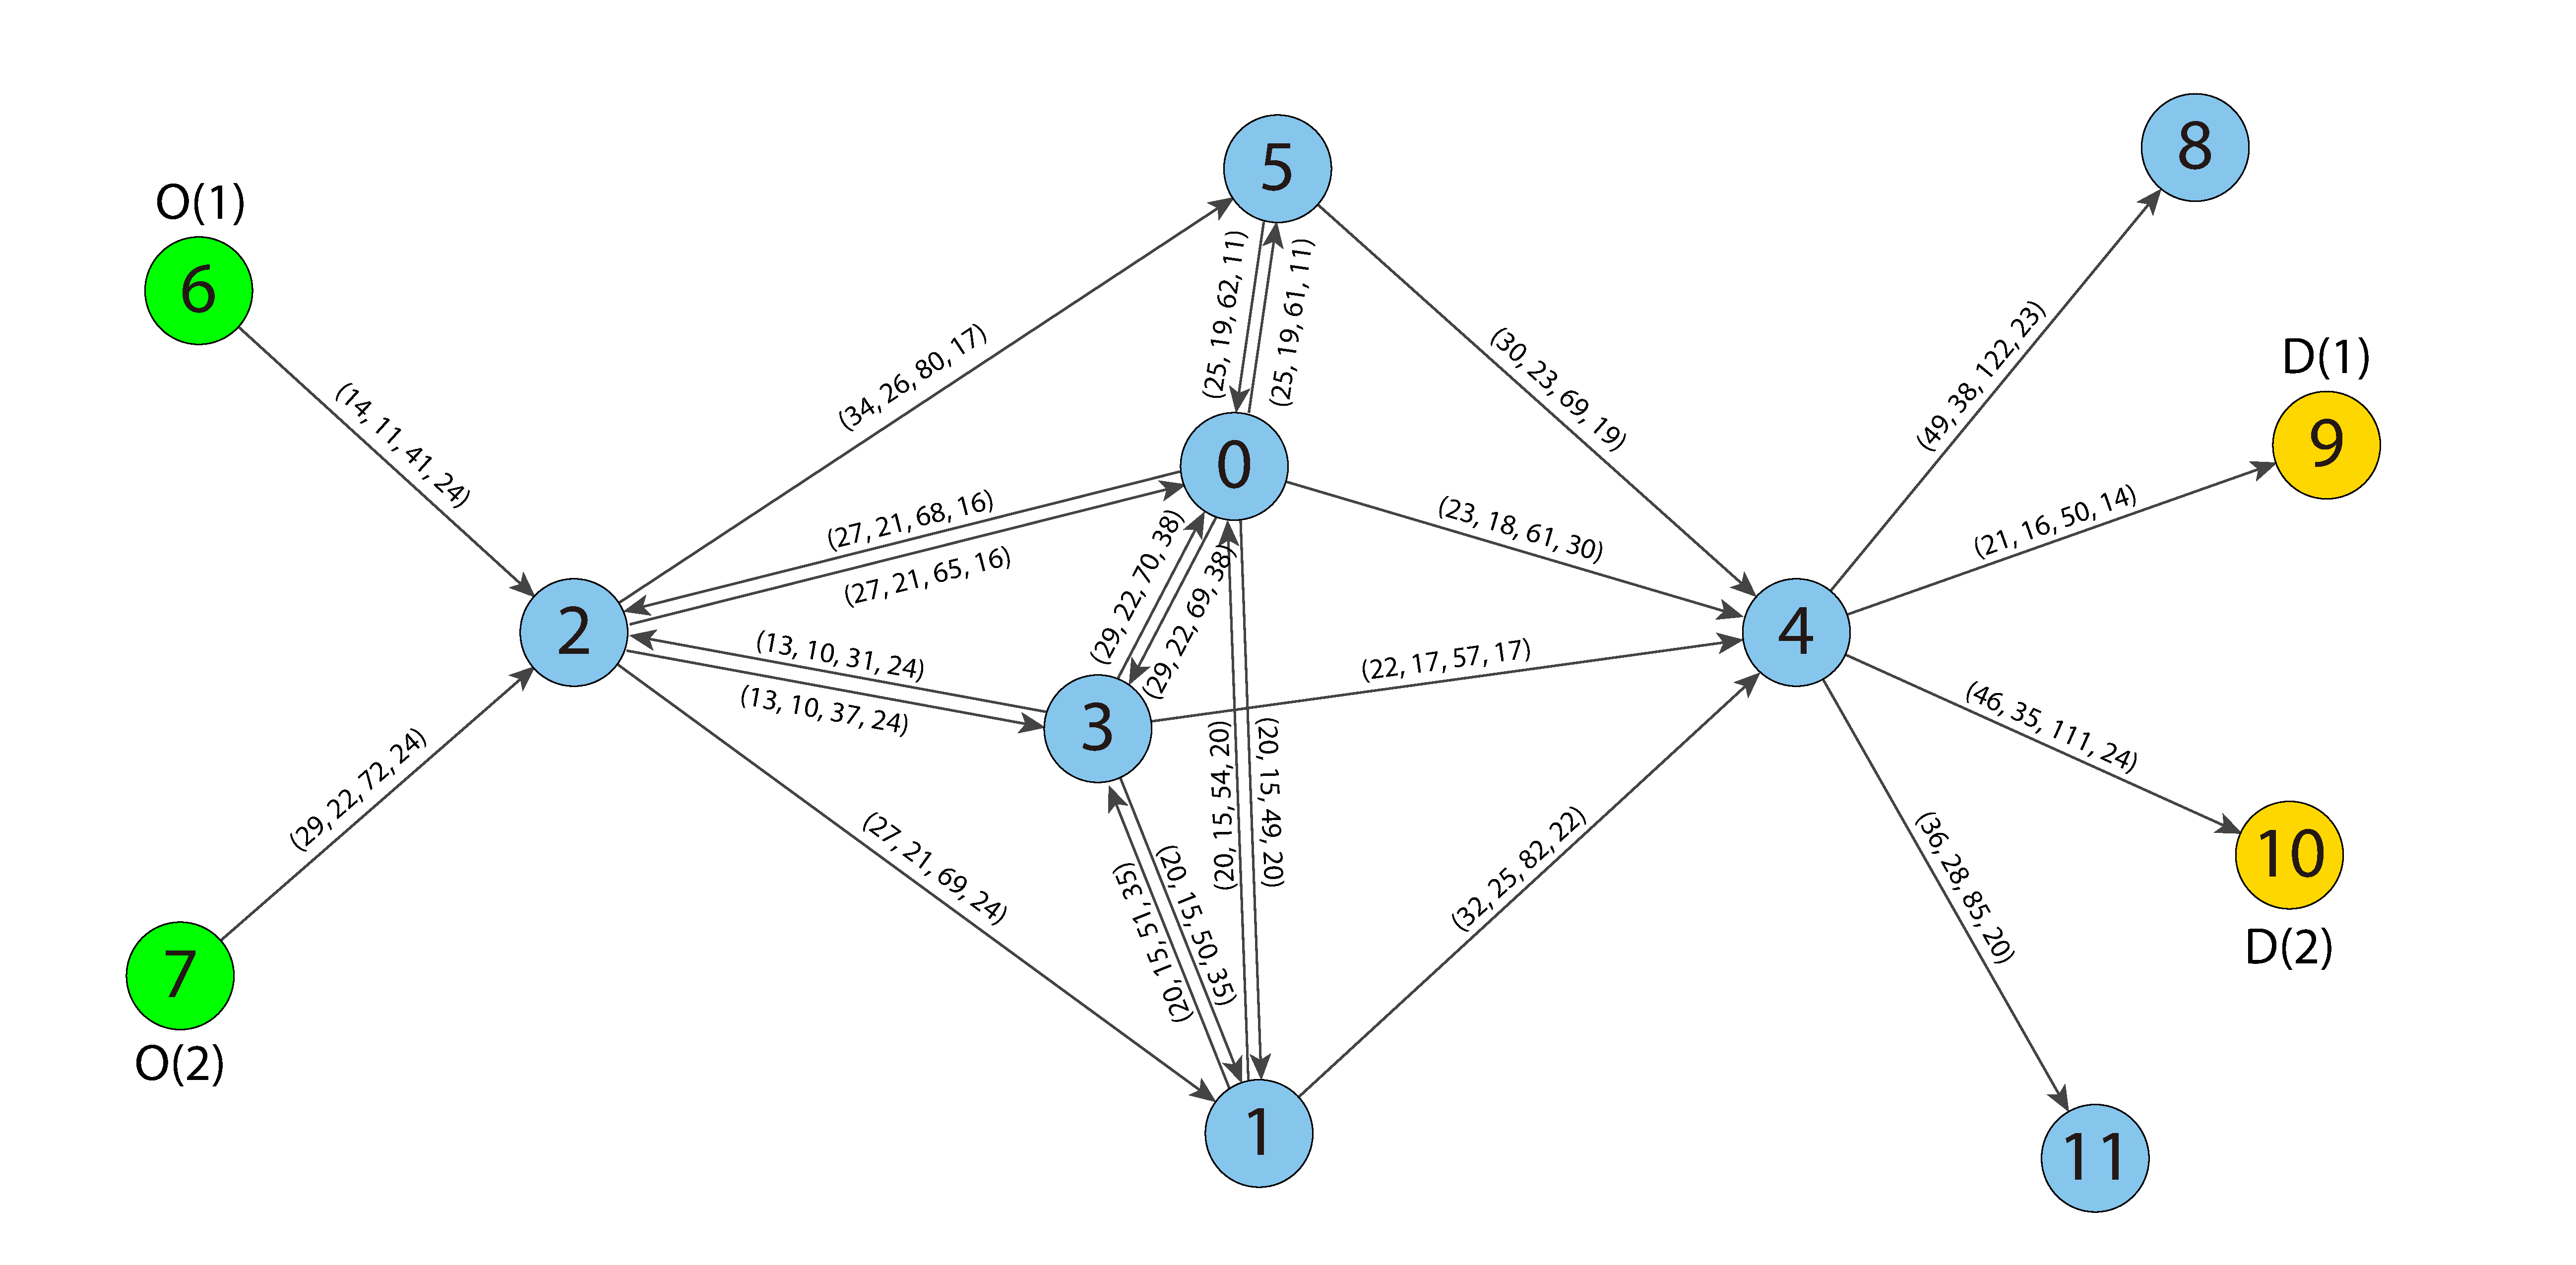
\includegraphics[width=\textwidth]{figures/Reinforcement/Example2.pdf}
    \caption{Example 2: a tuple on the edge represents $(c_{ij}^1, c_{ij}^2, f_{ij}, u_{ij})$}
    \label{fig:Example2}
\end{figure}
\clearpage

We define a global state $S_t \in \mathcal{S}$: $$S_t = (i_1, i_2, \boldsymbol{u}^t, \boldsymbol{y}^t) \in V \times V \times \mathbb{R}^{|E|} \times \{0,1\}^{|E|} = \mathcal{S},$$ with the following notations:
\begin{itemize}
    \item $i_k \in V$ for $k = 1,2$ is a node at which the agent $k$ is currently located
    \item $\boldsymbol{u}^t$ is a $|E|-$dimensional vector of $\{u_{(i,j)}^t\}_{(i,j)\in E}$, where $u_{(i,j)}^t$ is a remaining capacity of an edge $(i,j) \in E$ at time step $t$
    \item $\boldsymbol{y}^t$ is a $|E|-$dimensional vector of $\{y_{ij}^t\}_{(i,j)\in E}$, where $y_{ij}^t$ is a design variable on $(i,j)$ at time step $t$.
\end{itemize}

For $k = 1,2$, an action $A_t^{(k)}(s) \in \mathcal{A}^{(k)}$ available in state $S_t = (i_1, i_2, \boldsymbol{u}^t, \boldsymbol{y}^t)$ is to choose an edge $(i_k, j_k)$ where $$j_k \in \{j_k \in V \ | \ (i_k, j_k) \in E \text{ and } d^k \leq u^t_{i_k j_k}\} = \mathcal{A}^{(k)}(S_t).$$

%We note that it is hard to define how to calculate the remaining capacity when there exists an edge that has been visited by the same agent more than two times. To prevent this situation, we let agents follow a path only, meaning that it is not allowed to select an edge $(i_k,j_k)$ whose target node $j_k$ has already been visited by the agent $k$.

In order that the capacity constraints \eqref{eq:Capacity constraints} are not violated, we add the following setup. At each time step, if there exists an edge whose capacity constraint is violated by agents' actions, the agents who cause this situation bounce back to their original position. For example, at time step $t$, if two agents simultaneously choose the same edge $(i,j)$ whose current capacity $u_{ij}^t$ is less than the sum of their quantity $d^1 + d^2$, then both agents stay in the node $i$ at the next time step $t+1$.

We now discuss a reward function for \hyperref[fig:Example2]{Example 2}. Since we consider a deterministic environment, we have:
$$r(s,z) = r(s, z, s'),$$
where $s' = (i_1', i_2', \boldsymbol{u}', \boldsymbol{y}')= \tau(s,z)$. Then we define a reward function as follows:
\begin{align}
    r(s,z,s') = - \left(r_f + \sum_{k=1}^
    Kr_k\right),
\end{align}
where\footnote{Here $\{y_{ij}'\}_{(i,j)\in E}$ denote elements of $\boldsymbol{y}'$} \begin{align}
    r_f &= \sum_{(i,j)\in E}(y'_{ij}-y_{ij}) \cdot f_{ij}\\
    r_k &= \begin{cases}
    \beta &\text{if } i_k = i_k'\\
    c_{i_k i_k'}\cdot d^k &\text{if } i_k \neq i_k'
    \end{cases} \quad \text{for all } k \in \mathcal{K}
\end{align}
with a punishment factor $\beta \in \mathbb{R}_{>0}$.
\clearpage
\section{Value-based Methods}
In this section, we introduce


\subsection{Independent Q-learning}
Independent Q-learning (IQL) (\citeauthor{tan1993multi} \cite{tan1993multi}) is one of the pioneering approach to learning in the multi-agent settings. In IQL, each agent acts independently while the rest of agents are considered as part of the environment. In other words, each agent cannot observe other agents' action choice, while the reward function and the state-transition function depend on both a global state and actions of all agents. Thus, the environment becomes non-stationary from the perspective of each agent.

\subsection{Distributed Q-learning}
Distributed Q-learning (\citeauthor{lauer2000algorithm} \cite{lauer2000algorithm}) is an extension of IQL, where learning is distributed among agents. One can also say that the learning is decentralized. Let us split a policy $\Pi$ into $M$ agent-individual policies $\pi^{(m)}(s): \mathcal{S} \rightarrow \mathcal{A}^{(m)}$ with $\Pi(s) = (\pi^{(1)}(s), \dots, \pi^{(m)}(s), \dots,  \pi^{(M)}(s))$. Then a decentralized learning means that we learn each policy $\pi^{(m)}$ individually. \citeauthor{lauer2000algorithm} \cite{lauer2000algorithm} consider cooperative Markov games in their paper, and prove that their algorithm can find an optimal policy $\Pi_\ast$ in deterministic environments.

The main idea of distributed Q-learning is to properly compress the information of the central Q-table $Q(s,z)$ of size $|\mathcal{S}| \times |\mathcal{Z}|$ to the $M$ small, agent-individual tables $q^{(m)}(s,a^{(m)}$ of size $|\mathcal{S}| \times |\mathcal{A}^{(m)}|$.



The distributed Q-learning is comprised of two iteration rules. The first one is an algorithm that creates the small, agent-individual $q^{(m)}$-tables, describes as:
\begin{align}
    q_0^{(m)} &= 0\nonumber\\
    q_{t+1}^{(m)}(s,a^{(m)}) &=
    \begin{cases}
        q_t^{(m)}(s,a^{(m)}) &\mbox{if } s\neq S_t \text{ or }\\ & \quad a^{(m)}\neq A_t^{(m)}\\
    \max\{q_t^{(m)}(s,a^{(m)}), \\ \qquad r(S_t,Z_t) + \beta \cdot \underset{\tilde{a}^{(m)}\in\mathcal{A}^{(m)}}{\text{max}}q_t^{(m)}(S_{t+1}, \tilde{a}^{(m)})\} & \mbox{otherwise,}
    \end{cases}
\end{align}
where $A_t^{(m)}$ is agent $m$'s action choice at time step $t$, and $Z_t$ is the joint action of all agents at time step $t$.


The other one is an update rule for each agent-individual policy $\pi^{(m)}$.
\begin{align}
\pi_0^{(m)}(s) &\in \mathcal{A}^{(m)} \text{ arbitrarily }\nonumber\\
\pi_{t+1}^{(m)}(s) &= \begin{cases}
\pi_t^{(m)}(s) &\mbox{if }s\neq S_t \text{ or }\\
& \underset{a^{(m)}\in\mathcal{A}^{(m)}}{\text{max}}q_t^{(m)}(s,a^{(m)}) = \underset{a^{(m)}\in\mathcal{A}^{(m)}}{\text{max}}q_{t+1}^{(m)}(s,a^{(m)})\\
a_t^{(m)} &\mbox{otherwise}
\end{cases}
\end{align}




\section{Policy-based Methods}









